Initial attempts to create models describing fission gas release were based on empirical correlations. Analyses performed with such models are limited in scope since they depend on a limited set of experimental observations. Simulations with conditions set outside the realm of the experimental data are extrapolating and therefore unreliable, especially when it is acknowledged that the input parameters to the fission gas release models have high uncertainty. To this end, a physics-based fission gas release model was developed by Pastore et. al \cite{Pastore3}. Physics based models are based on the solution of partial differential equations describing the various processes in fission gas release such as fuel swelling and diffusion of gas bubbles to the rod free volume. 

There are two primary physical processes that lead to fission gas release into the rod free volume. Both processes involve the formation of Xenon and Krypton gas bubbles along UO$_2$ grain boundaries. In athermal gas release, which occurs at relatively low operating reactor temperatures, the diffusion of gas bubbles from within the fuel grains is negligible. However, in athermal gas release bubbles along fuel grain surfaces are able to escape into the rod free volume through the release mechanisms of recoil and knockout \cite{Pastore1}. At high temperatures fission gas release is dominated by thermal release, which involves the coupling of several physical processes. In thermal release Xenon and Krypton gas atoms formed within fuel grains diffuse towards the grain boundaries through trapping-in and irradiation-induced resolution \cite{Pastore3}. Additional gas bubbles appear onto grain boundaries through sweeping due to grain growth. As more and more gas bubbles diffusion towards grain boundaries the bubbles experience growth and ultimately coalesce. Eventually, tunnel networks form that provide a means for fission gases to escape into the rod free volume. The internal pressure causing bubble growth can be subdued by hydrostatic stress from the rod internal pressure and pellet/cladding contact pressure. A primary motivation for developing a physics-based fission gas release model is to accurately describe the interplay between these opposing forces \cite{Pastore3}.    

The physics-based models for athermal and thermal fission gas release are given mathematical treatments in the proceeding sections. The implementation of the physics-based fission gas release model by Pastore et. al., namely \ac{SIFGRS}, is implemented in the Bison code and utilized in this research. The implementation is validated in \cite{Pastore1}, \cite{Pastore2}, \cite{Perez}, and \cite{Pastore}. Note that the models on which the \ac{SIFGRS} implementation is based on is kept relatively simple in order to provide timely estimates of fission gas release in the computationally expensive, finite-element based Bison code. The relative simplicity of the models is justified considering the large uncertainties in both fuel performance modeling codes and model parameters in the fission gas release model \cite{Pastore2} \cite{Lassmann}. 

The primary challenges of modeling thermal fission gas release are in describing the diffusional process of fission gases to grain boundaries and the resulting bubble growth and coalescence. As mentioned previously, the thermal release model is intended to be relatively simple, and as such, makes several assumptions that are in contrast to the current understanding of materials science. Upon reaching a fuel grain boundary fission gas atoms can be thrust back into the grain by irradiation. Such behavior is neglected in the proceeding model. Further, the complexity of grain edges, most notably triple grain junctions, are completely neglected. In addition, the initial concentration of grain face bubbles is static, which is not entirely correct because new bubbles will form during any irradiation process. Bubbles are also assumed to absorb any gas atoms arriving at grain faces. Finally, all grain face bubbles are assumed to have the same size and shape \cite{Pastore1}.  

Fission gas bubble growth is known to result from two channels. First, growth occurs due to absorption of vacancies caused by a pressure differential between the bubble's expansion and external forces acting on the bubble. Second, bubble growth is accelerated due to the diffusional process bringing gas atoms from the inner fuel grain to the grain faces. To this end, bubble growth rate can be described as,
\begin{equation}
\label{eq:bubble_growth}
 \frac{dV_{gf}}{dt} = \omega\frac{dn_g}{dt} + \Omega_{gf}\frac{dn_v}{dt}  
\end{equation}  
where $V_{gf}$ is the bubble volume, $n_v$ is the number of vacancies per bubble, and $n_g$ is the number of fission gas atoms per bubble. The first term in Eq. \ref{eq:bubble_growth} describes the contribution from diffusional gas atoms while the second term describes absorption of vacancies. The factors $\omega$ and $\Omega_{gf}$ are respective proportionality constants commonly described in the literature as Van Der Waal's' volume  of a fission gas atom and the vacancy volume in grain boundary bubbles. The term due to diffusional gas atoms is obtained by solving the diffusion equation in spherical geometry for the concentration of intra-granular gas atoms $C_{ig}$,
\begin{equation}
\label{eq:bubble_diffusion}
 \frac{dC_{ig}}{dt} = \frac{b}{b+g}D_s \frac{1}{r^2} \frac{\partial}{\partial r} \left(r^2 \frac{\partial C_{ig}}{\partial r} \right) +\beta.
\end{equation}
The effective diffusion coefficient in Eq. \ref{eq:bubble_diffusion}, which regulates the rate at which gas atoms in a UO$_2$ lattice diffuse from fuel grain to face, consists of several components. The factor $g$ represents the trapping parameter while $b$ is the resolution parameter. Together, the ratio $b/(b+g)$ is the fraction of all intra-granular gas atoms that can potentially diffuse towards the grain boundary \cite{Pastore3}. The final component in the effective diffusion coefficient is the intra-granular gas atom diffusion coefficient $D_s$, which carries the classic interpretation of a diffusion coefficient. The source term in Eq. \ref{eq:bubble_diffusion} is the rate at which gas is generated. 

Changes in vacancy absorption and emission, the second term in Eq. \ref{eq:bubble_growth}, is proportional to the pressure differential of the gas bubble. If $n_v$ is the vacancy number in a bubble then the time rate of change of $n_v$ is given by,
\begin{equation}
\label{eq:vacancy_change}
 \frac{dn_v}{dt} = \frac{2\pi D_v \delta_g}{kTs}\left(p - p_{eq}\right).
\end{equation}    
The internal pressure of the gas bubble can be expressed using Van Der Waal's equation,
\begin{equation}
\label{eq:interal_gas_pressure}
 p = \frac{kT}{\Omega_{gf}} \frac{n_g}{n_v}
\end{equation}
where $k$ is Boltzman's constant and $T$ is temperature. The pressure $p_{eq}$ acting on the bubble is given as the difference between the bubble surface tension and the hydrostatic stress $\sigma_h$ of the surrounding medium. More formally,
\begin{equation}
\label{eq:external_gas_pressure}
 p_{eq} = \frac{2\gamma}{R_{gf}} - \sigma_h
\end{equation} 
where $R_{gf}$ is the bubble radius of curvature. The factor $\gamma$ is the surface tension, which is also commonly referred to as the UO$_2$/gas specific surface energy. The surface tension parameter strongly affects the kinetics of bubble growth \cite{Swiler3}. To solve for the vacancy number in Eq. \ref{eq:vacancy_change} the grain boundary diffusion layer thickness $\delta_g$ is needed in addition to the vacancy diffusion coefficient $D_v$. The factor $s$ in Eq. \ref{eq:vacancy_change} is closely related to the grain face fractional coverage \cite{Pastore1}. At this point all the elements are in place to model bubble growth using Eq. \ref{eq:bubble_growth}.  

As bubbles increase in size along grain boundaries they will eventually run into each other and coalesce, as exemplified in Fig. \ref{fig:bubble_coalesce}. Under the premise of conservation of total bubble volume, the relationship between bubble number density $N_{gf}$ and the projected bubble area along the grain face $A_{gf}$ can be expressed as \cite{Pastore3},
\begin{equation}
\label{eq:bubble_coalesecence}
 \frac{dN_{gf}}{dt} = -\frac{6N_{gf}^2}{3+4n_{gf}A_{gf}} \frac{dA_{gf}}{dt}.
\end{equation}

\begin{figure}
\caption{\label{fig:bubble_coalesce}
Bubble coalesce on a fuel grain face from the AGR/Halden Ramp Test Programme\cite{White}.}
 \begin{center}
  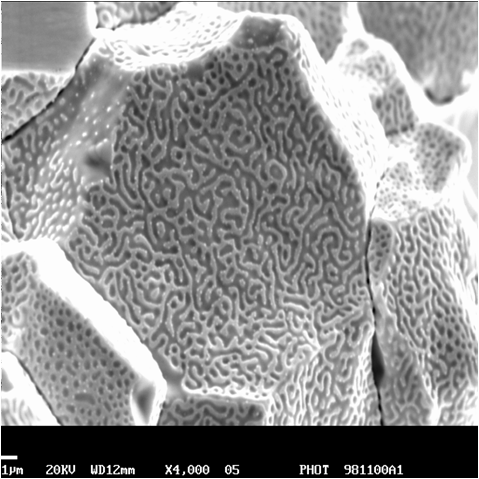
\includegraphics[scale=1.]{./Slides/fgr_1.png}
 \end{center}
\end{figure}
The bubble number density is obtained by solving \ref{eq:bubble_growth}. The processes of bubble growth and coalescences along fuel grain boundaries lead to fission gas release once certain saturation criteria have been met. Let $F_c = N_{gf}A_{gf}$ denote the fraction of a grain face covered by bubbles. The saturation condition holds when the time rate of change of $F_c$ is static. When the saturation condition holds, the relation between bubble number density and projected grain face area can be reformulated as,
\begin{equation}
\label{eq:bubble_coalesecence_sat}
 \frac{dN_{gf}}{dt} = -\frac{N_{gf}}{A_{gf}} \frac{dA_{gf}}{dt}.
\end{equation}
Only when the saturation condition has been reached can fission gas escape into the rod free volume. Once the saturation condition is met, Eq. \ref{eq:fgr_rate} can be used to model the concentration of gas atoms released per unit grain face. 
\begin{equation}
\label{eq:fgr_rate}
 \frac{d\psi_{thr}}{dt} = n_g \frac{1}{2} \frac{2N_{gf}A_{gf} - 3}{4N_{gf}A_{gf}} \frac{dN_{gf}}{dt}
\end{equation}      
where $n_g$ is the number of fission gas atoms per grain face bubble. The authors in \cite{Pastore3} argue that the process of fission gas release works strictly to reduce the bubble gas content and size but not concentration. 

While \ref{eq:fgr_rate} is useful for quantifying fission gas release, a more useful metric is the concentration of gas atoms release per unit fuel volume $C_{thr}$. The metric $C_{thr}$ is related to $\psi_{thr}$ through the proportionality constant equal to the grain surface to volume ratio \cite{Pastore2}, as expressed in \ref{eq:fgr_rate_final}.
\begin{equation}
\label{eq:fgr_rate_final}
 \frac{dC_{thr}}{dt} = \frac{3}{r_{gr}}\left(1 - P_f\right) \frac{d\psi_{thr}}{dt}
\end{equation} 
In Eq. \ref{eq:fgr_rate_final} the factors $r_{gr}$ and $P_f$ represent the fuel grain radius and fuel porosity, respectively. Both of these parameters are omnipresent in fuel performance modeling and have a significant effect on fission gas release values. As the fuel grain radius increases during irradiation the grain surface to volume ratio decreases. Consequently, fuel grain faces generally are less able to hold fission gases \cite{Pastore1}. In addition, an increase in fuel grain radius implies a larger travel distance for the fission gases to reach the grain face, per Eq. \ref{eq:bubble_diffusion}. Furthermore, in the phenomenon of grain boundary sweeping additional fission gases are swept to grain faces resulting from fuel grain growth, and specifically, moving grain boundaries. The fuel grain radius is the determinant in governing the fraction of intra-granular gas atoms get swept to the boundaries, as evidenced in Eq. \ref{eq:grain_boundary_sweeping}.
\begin{equation}
\label{eq:grain_boundary_sweeping}
 f = \frac{r_{gr,i}^3 - r_{gr,i-1}^3}{r_{gr,i}^3}
\end{equation}    
The $i$ in Eq. \ref{eq:grain_boundary_sweeping} refers to the $i^{\mbox{th}}$ time-step since grain boundary sweeping makes time-dependent contributions. 

In the Bison implementation of the fission gas release model described above, integral fission gas release values are reported. Being a finite element code, Bison computes the gas release at each integration point. The ratio of  total fission gas released into the rod free volume to the total fission gas generated at each integration point is the quantity of interest in this thesis. Also, note that since Bison makes time-dependent calculations and the \ac{SIFGRS} model accepts parameter values such as temperature from the greater code, how to go about a parametric or sensitivity analysis is not straight forward. To this end, scaling factors have been introduced into \ac{SIFGRS}. At each time-step in a Bison simulation the a set of predetermined scaling factors are applied to their corresponding parameters \cite{Pastore2}. As discussed in \cite{Pastore2}, the existing framework in Bison for propagating uncertainty values is not ideal. For example, to accurately asses the affect of temperature on fission gas release the material properties directly determining temperature fields should be parameterized.    

As a final note, due to the relatively high temperatures involved in the Ris\o~AN3 power ramp experiment athermal fission gas release is mostly trumped by its thermal counterpart. Nevertheless, for completeness the equations implemented in Bison for modeling the recoil-and-knockout phenomena leading to athermal gas release is included in Eq. \ref{eq:athermal_release}. 
\begin{equation}
\label{eq:athermal_release}
 \frac{dC_{atr}}{dt} = \frac{yF}{4} \left( \frac{S_g}{V} \mu_f +2 \frac{S_t}{V}\mu_{U,ko}\right)  
\end{equation}
The parameters $y$ and $F$ are the yield of fission gases and fission rate density, respectively. Also, $S_g$, $S_t$ and $\mu_{U,ko}$ are the geometric surface area of the fuel, total fuel surface area, and range of higher-order knock-on in uranium oxide \cite{Pastore2}. 



